\documentclass[10pt,twoside,slovak,a4paper]{article}
\usepackage[slovak]{babel}
\usepackage[IL2]{fontenc}
\usepackage[utf8]{inputenc}
\usepackage{graphicx}
\usepackage{url} 
\usepackage{hyperref} 
\usepackage{cite}
\pagestyle{headings}

\title{Objavovanie histórie pomocou hier\thanks{Semestrálny projekt v predmete Metódy inžinierskej práce, ak. rok 2022/23, vedenie: Ing. Igor Stupavský}} 

\author{Michal Červeňan\\[2pt]
	{\small Slovenská technická univerzita v Bratislave}\\
	{\small Fakulta informatiky a informačných technológií}\\
	{\small \texttt{xcervenan@stuba.sk}}
	}

\date{\small 14. október 2022}

\begin{document}

\maketitle

\begin{abstract}
Aj keď sú videohry novodobé médium, ktoré sa objavilo len zopár desiatok rokov späť, tak aj ony môžu pomôcť nahliadnuť do tajov minulosti
\end{abstract}



\section{Úvod}

Hry sú médium ktoré umožňuje autorom využiť ich kreativitu na maximum. A tak vedia vzniknúť fascinujúce svety s velkým množstvom nám neznámeho, to ale neznamená že sa nedá z hier aj niečo naučiť. A aj keď väčšina herných príbehov je vymyslená, tak si z nich vieme odniesť aspoň niečo o Historii. Podľa výberu hry sa vieme dozvedieť napríklad: spôsob života v danom obdobý, podstatu historických udalostí alebo aj príbeh určitej postavy ~\ref{moj typ}




\section{Diagram práce na projekte} \label{diagram}
\begin{center}
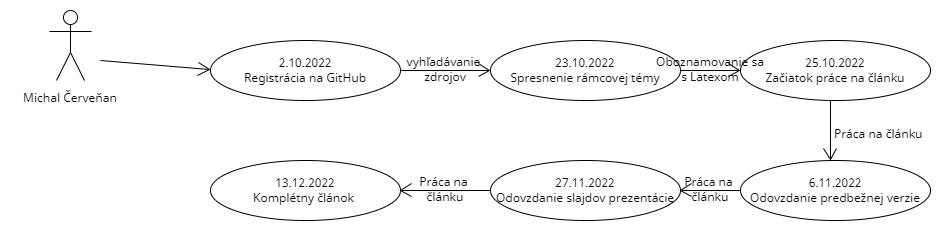
\includegraphics[width=.6\textwidth]{diagram.png}
\end{center}
\section{Experiment v Číne} \label{cina}
V rokoch 2009-2010 v číne vytvorili hru o troch mongoľských vpádoch, a zavesili ju na stránku www.hkedcity.net kde si ju môhli študenti zadarmo zahrať.

V máji 2010 bola hra už rok dostupná. Počet hráčov prvého vpádu bol 1329\cite{Yan2010}, druhý si zahralo 395 hráčov\cite{Yan2010}, a 353 \cite{Yan2010} bol počet hráčov tretieho vpádu. Následne bol vykonaný priezkum ktorého sa zúčastnilo 428 hráčov z toho 58\verb|%| mužov a 42\verb|%| žien\cite{Yan2010}.70\verb|%| zúčastnených študentov si myslí že sa naučili históriu vďaka tejto hre\cite{Yan2010}. Učitelia venovali 20 minút z hodiny aby si mohli zahrať túto hru\cite{Yan2010}. A podla nich to študentom zlepšilo postoj k učeniu zaćali dávať väčší pozor a zaujímali sa viac o hodiny\cite{Yan2010}.





\section{Hry ktoré môžu dopomôcť k učenie sa histórie} \label{moj typ}
Existuhe obrovské množstvo hier a tak som sa rozhodol vybrať zopár hier z ktorých sa dá dozvedieť niečo o minulosti
\begin{enumerate}
\item Valiant Hearts: The Great War - rozpráva príbehy 4 postáv počas prvej svetovej vojny. Dozvedáme o významních bitkách prvej svetovej vojny, taktiež obsahuje dobové fotky,listy, atď. v podobe zberateľských predmetov.
\item Kingdom Come: Deliverance - hra z obdobia stredoveku. Obsahuje historické bitky, hrady,a iné české lokality , taktiež nám poodhaľý niečo o živote počas stredoveku, a  
\item Company of Heroes 2 - strategická hra z obdobia druhej svetovej vojny. Môžeme sa dozvedieť udalosti niektorých významnejších bitiek a niečo o technike z druhej svetovej vojny
\item Age of Empires - séria strategických hier z obdobia stredoveku. Sú v nej obsiahnuté historické bitky a príbehy niektorých víznamních postáv

\end{enumerate}


\section{Záver} \label{zaver} 



\bibliography{Zdroje.bib}
\bibliographystyle{plain}
\end{document}
